\chapter{Results and Discussion}
\label{chap:results}

\section{Experimental Setup}
\label{sec:setup}

The evaluation used 15 open-source C repositories. Each project ran through clang-tidy, the custom libclang scanner and the V781 pattern detector. Only repositories producing at least one qualifying alert made it into the set. No repository-specific configuration or handler tuning happened at any stage. The projects cover a wide variety of C software: parsers, text editors, relational databases, game engines, network daemons, a reverse engineering framework, an image library, a time-series database, an interactive fiction interpreter and a language runtime. Table~\ref{tab:repos} lists all repositories with their categories.

{%
\renewcommand{\arraystretch}{1.3}
\setlength{\tabcolsep}{5pt}
\begin{table}[ht]
\caption{Repositories used in the real-world evaluation.}
\label{tab:repos}
\centering
\begin{tabular}{|l|l|}
\hline
\textbf{Repository} & \textbf{Category} \\
\hline
orangeduck/mpc          & Parser combinator library \\
bartp5/libtexprintf     & printf/\TeX{} formatting library \\
libretro/libretro-prboom & Game engine (DOOM port) \\
n-t-roff/heirloom-doctools & Document formatting tools \\
TheAlgorithms/C         & Algorithm implementations \\
cesanta/mongoose        & Embedded web server \\
radareorg/radare2       & Reverse engineering framework \\
vim/vim                 & Text editor \\
netdata/netdata         & System monitoring daemon \\
angstsmurf/spatterlight & Interactive fiction interpreter \\
sqlite/sqlite 3.41.2    & Embedded relational database \\
sqlite/sqlite 3.42.0    & Embedded relational database \\
glennrp/libpng          & PNG image library \\
taosdata/TDengine       & Time-series database \\
python/cpython 3.13.3   & Python language runtime \\
\hline
\end{tabular}
\end{table}
}

The evaluation environment consisted of Python~3.11.9, libclang~18.1.1, clang-tidy~21.1.8 and GCC/MinGW~6.3.0 on Windows~11. Each repository was cloned at a fixed commit and scanned to produce an alert JSON file, which then went through the pipeline. Each output directory yielded PASS, SKIP and FAIL classifications. No manual steps occurred between scanning and classifying the 372 alerts.

\section{Repair Results}
\label{sec:repair_results}

Table~\ref{tab:results} summarises the outcome breakdown per pattern. Of the 372 alerts processed, the tool repaired 328 of the 329 non-skipped instances. That is a 99.7\% accuracy rate. When the 43 skips enter the denominator, the overall fix rate drops to 88.2\%. A skipped alert is not a failure. Each left the source file unchanged, which is the safe outcome. At 88.2\%, every skip counts as a non-repair, so it is a conservative lower bound.

{%
\renewcommand{\arraystretch}{1.3}
\begin{table}[ht]
\caption{SafeRepair repair results by pattern.}
\label{tab:results}
\centering
\begin{tabular}{|l|r|r|r|r|r|r|}
\hline
\textbf{Pattern}         & \textbf{Alerts} & \textbf{PASS} & \textbf{SKIP} & \textbf{FAIL} & \textbf{Rate} & \textbf{Ovr. Rate} \\
\hline
SUSP\_REALLOC            & 180 & 168 & 12 & 0 & 100\% &  93\% \\
MISSING\_NULL            &  24 &   6 & 18 & 0 & 100\% &  25\% \\
INDEX\_CHECK             & 108 & 102 &  5 & 1 &  99\% &  94\% \\
SPRINTF\_UNBOUNDED       &  60 &  52 &  8 & 0 & 100\% &  87\% \\
\hline
\textbf{Total}           & \textbf{372} & \textbf{328} & \textbf{43} & \textbf{1} & \textbf{99.7\%} & \textbf{88.2\%} \\
\hline
\end{tabular}
\end{table}
}

The only deviations from a clean result are the MISSING\_NULL\_CHECK skip rate (75\%, driven by return-type ambiguity in the enclosing function) and the single INDEX\_CHECK failure; both are detailed in Section~\ref{sec:skip_fail}. The evaluation produced no false positives. Every handler either confirms the vulnerability in the AST and produces a fix, or declines to act.

\section{Generalisation Across Codebases}
\label{sec:generalisation}

Figure~\ref{fig:perrepo} shows the per-repository alert distribution sorted by total volume. Fix rates are consistent across all repository categories. SQLite and CPython~3.13 are the largest codebases in the set by size and internal complexity. Radare2 and Netdata contain significant platform-specific code with Linux-specific system headers. None required handler modifications or repository-specific configuration. \texttt{alert\_parser.py} handled all scanner-specific output format differences without any per-repository adjustment.

\begin{figure}[ht]
\centering
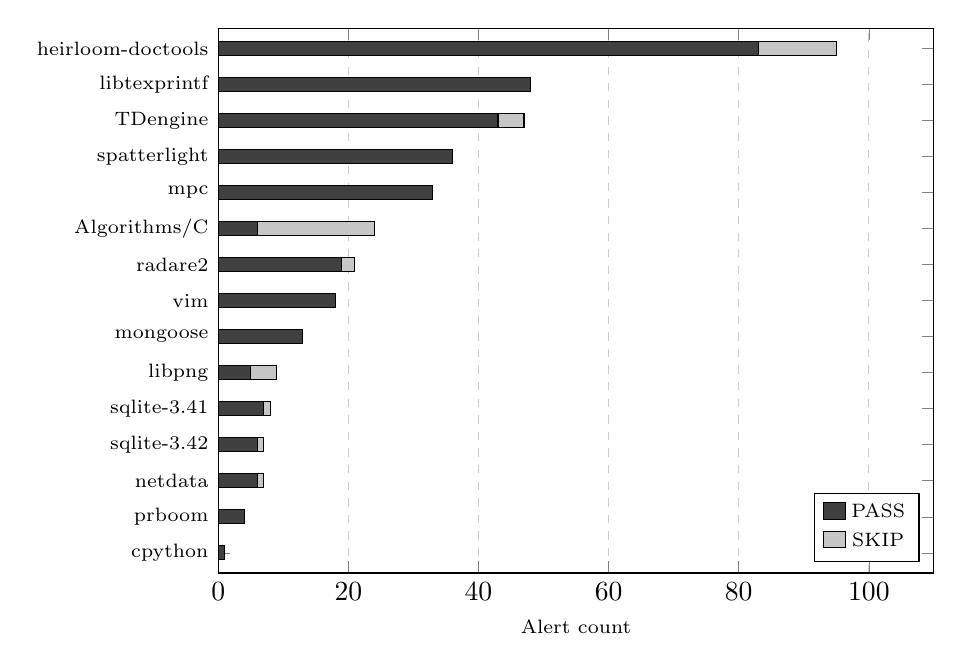
\begin{tikzpicture}
\begin{axis}[
  xbar stacked,
  bar width=5pt,
  width=0.88\columnwidth,
  height=8.5cm,
  symbolic y coords={
    cpython,prboom,netdata,sqlite42,sqlite41,
    libpng,mongoose,vim,radare2,algorithms,
    mpc,spatterlight,TDengine,libtexprintf,heirloom},
  ytick=data,
  yticklabels={
    cpython,prboom,netdata,sqlite-3.42,sqlite-3.41,
    libpng,mongoose,vim,radare2,Algorithms/C,
    mpc,spatterlight,TDengine,libtexprintf,heirloom-doctools},
  yticklabel style={font=\scriptsize},
  xmin=0, xmax=110,
  xlabel={\scriptsize Alert count},
  xmajorgrids=true,
  grid style={dashed, gray!40},
  enlarge y limits=0.04,
  legend style={at={(0.98,0.02)}, anchor=south east,
    legend columns=1, font=\scriptsize},
]
\addplot[fill=black!75, draw=black] coordinates {
  (1,cpython)  (4,prboom)    (6,netdata)   (6,sqlite42)
  (7,sqlite41) (5,libpng)    (13,mongoose) (18,vim)
  (19,radare2) (6,algorithms)(33,mpc)      (36,spatterlight)
  (43,TDengine)(48,libtexprintf)(83,heirloom)};
\addplot[fill=gray!45, draw=black] coordinates {
  (0,cpython)  (0,prboom)    (1,netdata)   (1,sqlite42)
  (1,sqlite41) (4,libpng)    (0,mongoose)  (0,vim)
  (2,radare2)  (18,algorithms)(0,mpc)      (0,spatterlight)
  (4,TDengine) (0,libtexprintf)(12,heirloom)};
\legend{PASS, SKIP}
\end{axis}
\end{tikzpicture}
\caption{Alert distribution across all 15 repositories, sorted by total volume. Dark bars show PASS; grey bars show SKIP. The single FAIL (vim/INDEX\_CHECK, 0.3\% of all instances) is excluded for clarity.}
\label{fig:perrepo}
\end{figure}


\section{Skip and Fail Analysis}
\label{sec:skip_fail}

\subsection{Skip Categories}

The 43 skips across the evaluation fall into four distinct causes:

\begin{itemize}
  \item \textbf{Macro-expanded pointers} account for all 12 heirloom-doctools skips in SUSPICIOUS\_\allowbreak REALLOC. At each flagged call site the realloc pointer passes through a preprocessor macro, so the handler cannot trace the token back to a named variable (see Section~\ref{sec:skip}).

  \item \textbf{Return-type ambiguity} explains 18 of the 24 MISSING\_NULL\_CHECK alerts, all in TheAlgorithms/C. The affected functions return struct types or non-standard error codes that do not map to any of the three supported sentinels.

  \item \textbf{Dynamically sized buffers} are behind the SPRINTF\_UNBOUNDED skips in libpng~(4) and TDengine~(4). The destination buffer is heap-allocated, so \texttt{sizeof}\allowbreak\texttt{(buf)} would return the pointer width instead of the allocation size.

  \item \textbf{Previously applied fixes.} A small number of alerts in SQLite and Radare2 pointed to lines already corrected in the scanned version by upstream developers. The pattern check fails for already-fixed code and the alert is skipped cleanly.
\end{itemize}

All 43 skips left the source file byte-for-byte unchanged. None produced a modified file with a wrong transformation.

\section{Discussion}

\subsection{Design Consequences of Right-or-Silent}

Zero false positives are not an empirical accident. The result follows directly from the design principle in Chapter~\ref{chap:methodology}. When a precondition check passes, the transformation is sound by the reasoning in Section~\ref{sec:handlers}. If it fails, the handler returns nothing. No handler has a code path that produces a modification when the pattern is unconfirmed.

The structure also makes patches auditable. Every SafeRepair patch traces back to a named rule with an explicit correctness argument. A developer reviewing a pull request can read the rule and verify the transformation in under a minute. A patch from a neural APR tool carries no such traceability. A reviewer must reconstruct the correctness argument from scratch.

\subsection{Comparison with Redemption}

Redemption by Svoboda et al.~\cite{b2} covers CWE-476, CWE-457 and CWE-561/1164 with the same deterministic AST-guided approach as SafeRepair. It is the most structurally similar prior work, achieving 94.4\% on one analyser across one codebase and over 80\% on average across two codebases. The main difference is in how each tool handles uncertain cases. Redemption applies repairs to probable false positives on the grounds that a superfluous null check is low-cost. SafeRepair refuses to act unless the AST confirms the pattern. Redemption suits workflows where a developer reviews every patch; SafeRepair fits automated pipelines. Their CWE sets overlap minimally, so both tools can run side by side.

\subsection{Comparison with Learning-Based Approaches}

VulRepair~\cite{b4} achieves 43.7\% exact match on C/C++ vulnerabilities across 1,754 projects; VulMaster~\cite{b3} reaches 20.3\% on a larger benchmark of 5,800 functions. Both generalise across arbitrary bug types without hand-coded rules, which is a genuine advantage for vulnerability classes with no concise structural pattern. The cost is GPU infrastructure and non-deterministic output. Neither tool provides a per-patch correctness guarantee. For the patterns SafeRepair targets, the fix is structurally determined from local context, and a rule-based handler is the right tool for that.

\subsection{Limitations}

The four skip categories in Section~\ref{sec:skip_fail} mark the current scope limits. Three are addressable. Resolving macro token sequences through libclang's token-expansion API before text rewriting would cut macro-expansion failures. Implementing INDEX\_CHECK as an AST-level operand swap instead of text-level search-and-replace would fix the vim FAIL and the residual macro failures. Dynamically sized buffer detection in SPRINTF\_UNBOUNDED requires pointer-provenance analysis to recover the allocation size. That is beyond local AST inspection and is a harder limit.

The fourth skip category, return-type ambiguity in MISSING\_NULL\_CHECK, has no clean solution within purely local analysis. Getting the correct error-return convention for an unfamiliar function requires interprocedural analysis or documentation lookup. Neither is available to a local handler. Skipping is the right call here.

The other gap is pattern coverage. CWE-476 (null pointer dereference at the dereference site) and CWE-415 (double free) both have local structural signatures that fit SafeRepair's architecture. Adding handlers for them would require no changes to the pipeline.
